\clearpage
\section{Simulador de radiología diagnóstica}
\label{result:xray}

%Para demostrar las capacidades del algoritmo propuesto de adaptar la posición de un paciente virtual con tasas de refresco interactivas, se desarrolló un simulador de radiología diagnóstica. 
El simulador de radiología diagnóstica desarrollado ofrece una plataforma de enseñanza y autoprendizaje de la radiología diagnóstica, donde el usuario puede cambiar la postura del paciente virtual y visualizar la proyección de manera interactiva. 
%
En la figura \ref{fig:simui2} se puede observar la \ac{IU} del simulador. En esta imagen se muestra al modelo \emph{ZygoteBody}$^{TM}$ situado decúbito supino en la mesa radiográfica. 
%En la zona central, se encuentra la vista de la escena 3D. En esta ventana, se podrá observar el modelo virtual cargado para la ocasión situado en una sala de radiología virtual. El usuario podrá utilizar el ratón para mover la perspectiva de la cámara y hacerse una idea de la escena virtual.
%En la esquina superior izquierda se sitúa el módulo de posicionamiento del modelo virtual. En esta división, el usuario puede seleccionar posturas previamente guardadas o almacenar nuevas posiciones. Además, puede seleccionar de manera individual cada articulación que disponga el modelo virtual. 
\begin{figure}[ht]
\centering
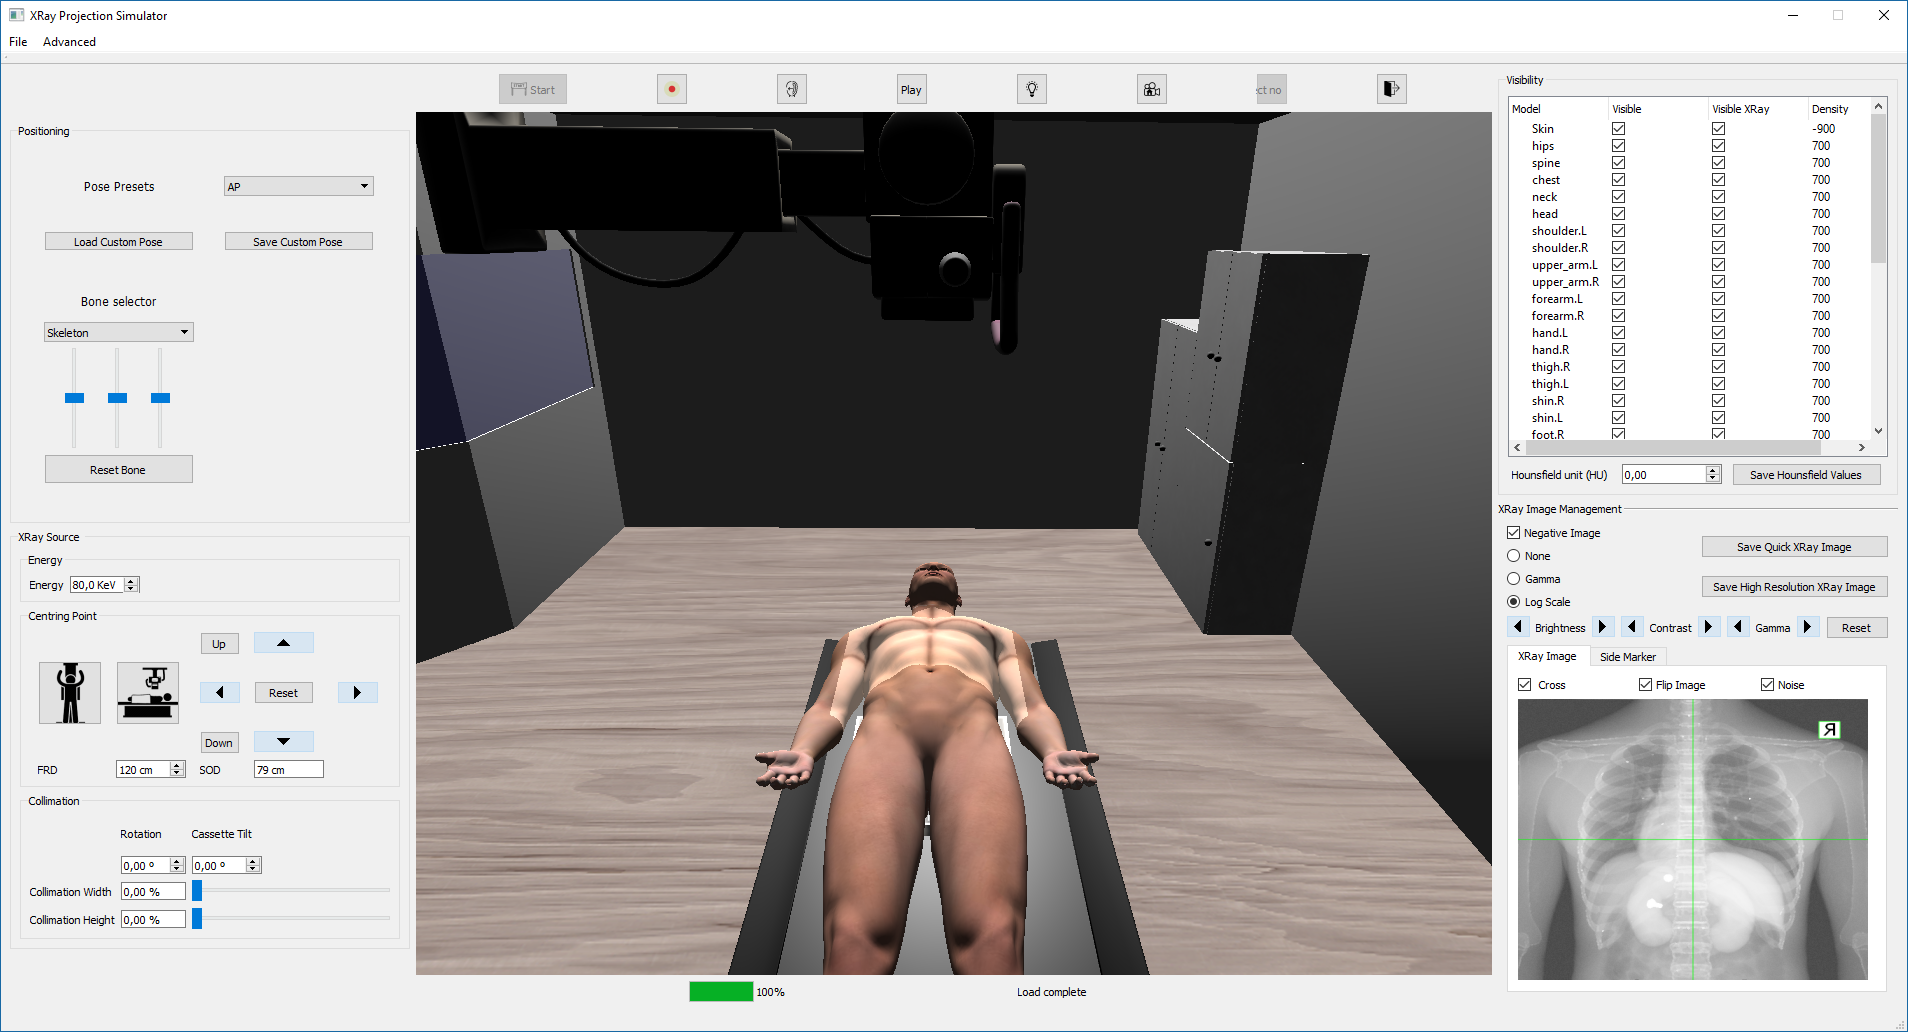
\includegraphics[width=0.95\linewidth]{IMG/simui.png}
\caption{\label{fig:simui2} Interfaz de usuario del simulador de radiología diagnóstica. }
\end{figure}

%En la esquina inferior izquierda, se puede observar todos los parámetros relacionados con la configuración del emisor de rayos X con el objetivo de conseguir una imagen radiográfica de calidad.
%Por otra parte, en la esquina superior derecha se encuentra una lista de los tejidos del paciente virtual que están disponibles. En esta lista, se puede esconder los tejidos bajo demanda o se puede cambiar sus propiedades químicas. Esta funcionalidad permite al usuario comprobar multitud de variaciones del modelo virtual cargado.

%Por último, en la esquina inferior derecha se puede observar la imagen de rayos X resultante de la posición del emisor en relación con el modelo virtual. En esta imagen se podrá apreciar la configuración de la colimación o de los distintos parámetros que definen un emisor de rayos X. Además, la imagen resultante puede ser modificada en cuanto a brillo, contraste, o filtros de imágenes. Esto ayuda al usuario a interpretar y entender la imagen al ocultar o resaltar detalles de la anatomía.




\subsection{Análisis previos}

Se han utilizado como modelos de entrada en el simulador los modelos presentados en la figura \ref{fig:models}. La flexibilidad del algoritmo propuesto permite incorporar cualquier paciente virtual externo, utilizando el preproceso descrito en la sección \ref{posing:preprocess}. En la figura \ref{fig:xraymodels} se muestran cuatro modelos anatómicos y su correspondiente radiografía de pecho.

\begin{figure}[ht]
    \begin{subfigure}[b]{0.24\linewidth}
        \centering
        {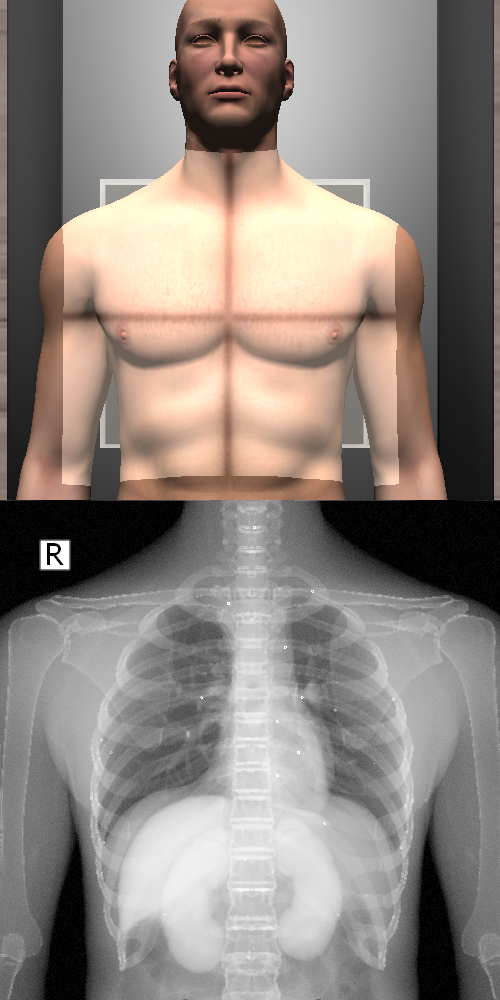
\includegraphics[width=\linewidth]{IMG/zygoteex.png}}
        \caption{\emph{ZygoteBody}$^{TM}$ Masculino.}
    \end{subfigure}
     \begin{subfigure}[b]{0.24\linewidth}
        \centering
        {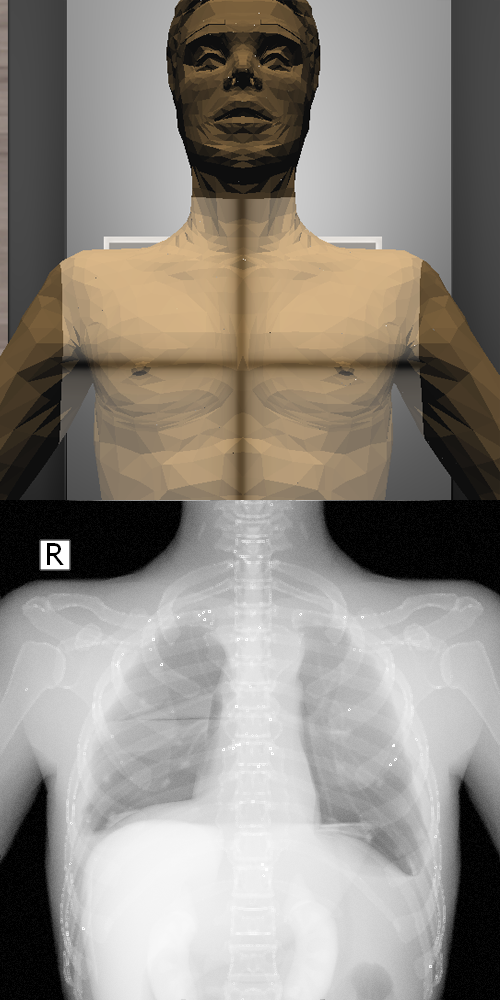
\includegraphics[width=\linewidth]{IMG/anaex.png}}
        \caption{\emph{Anatomium} Masculino.}
    \end{subfigure}
    \begin{subfigure}[b]{0.24\linewidth}
        \centering
        {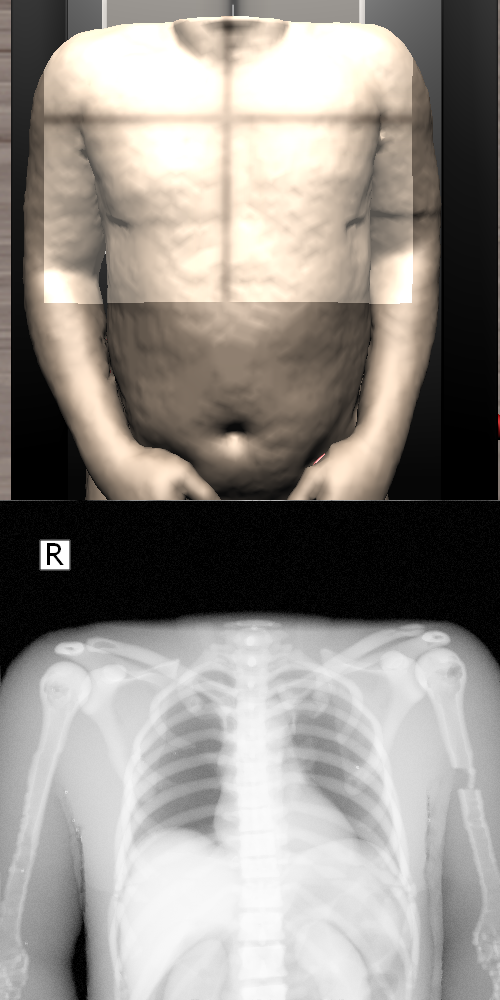
\includegraphics[width=\linewidth]{IMG/HVPex.png}}
        \caption{\emph{Segmented Inner Organs}\label{subfig:HVP}.}
    \end{subfigure}
     \begin{subfigure}[b]{0.24\linewidth}
        \centering
        {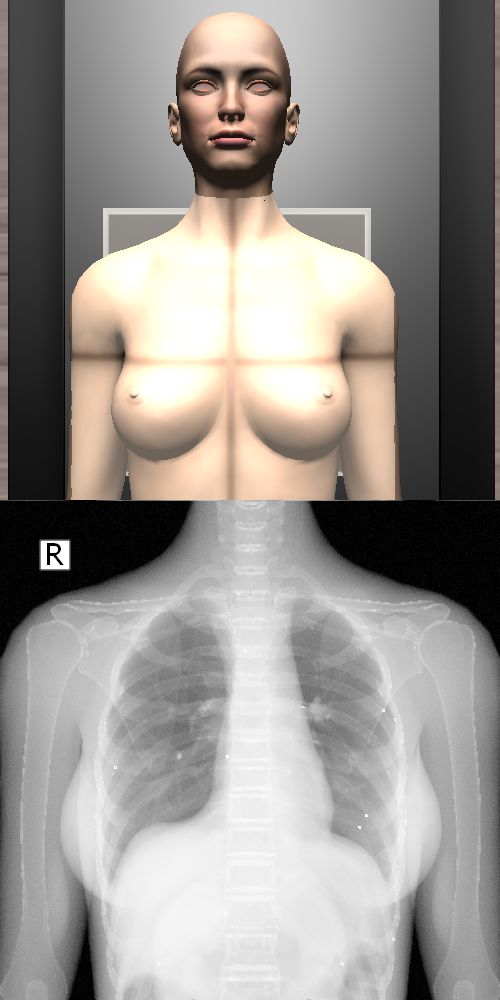
\includegraphics[width=\linewidth]{IMG/femaleex.png}}
        \caption{\emph{ZygoteBody}$^{TM}$ Femenino.}
    \end{subfigure}
    \caption{\label{fig:xraymodels} Modelos utilizados en el simulador de radiología diagnóstica.}
   \end{figure}
   
Como se puede observar, la calidad de la imagen radiográfica depende de la calidad del modelo del paciente virtual. %En concreto, los modelos comerciales necesitan una pequeña adaptación en los tejido óseos para mejorar el realismo de las imágenes. Los huesos presentan dos tipos de tejidos: 
% \begin{itemize}
%     \item Cortical: tejido denso que se encuentra en la capa externa de los huesos.
%     \item Trabecular: capa esponjosa que se encuentra en el interior de los huesos.
% \end{itemize}
En la mayoría de los casos, concretamente en los modelos comerciales, las mallas superficiales no representan correctamente los tejidos anatómicos del cuerpo humano. Esto, en el caso particular del simulador de radiología,  puede dar lugar a generación de imágenes poco realistas. 

En concreto, los modelos anatómicos comerciales utilizados, se proporciona solamente una representación  superficial de los huesos (cortical \footnote{Tejido denso que se encuentra en la capa externa de los huesos.}) y suelen ignorar los tejidos internos (trabecular\footnote{Capa esponjosa que se encuentra en el interior de los huesos.}). Como consecuencia de la ausencia de los tejidos internos, \emph{gVirtualXRay} no tiene en cuenta el interior y genera un tejido óseo homogéneo. 
Esta librería se basa en la funcionalidad de un trazador de rayos, por lo cual se calcula el recorrido del rayo a través de las estructuras anatómicas, entrando por la cara frontal del triángulo y saliendo por la cara trasera de otro triángulo de la misma malla. Este recorrido sirve para calcular la atenuación del rayo dependiendo de las propiedades físicas del material y de la longitud del recorrido del rayo. Al solo traspasar el tejido superficial, sin interacción con ninguna estructura interna, el tejido óseo aparece totalmente sólido en la imagen de rayos X resultante, dando lugar a una imagen no realista (ver fig.~\ref{subfig:nointernal}) que los médicos interpretan como una calcificación del hueso.

Con el objetivo de mejorar la representación de las zonas trabeculares, se ha desarrollado una pequeña modificación en el simulador. Cuando se carga el tejido óseo, se duplica su malla superficial, en la cual se invierten las normales y se encoge la geometría en esa dirección. De esta manera, se crea una estructura interna con una forma similar al hueso. En la figura ~\ref{fig:bonecompare} se puede observar la diferencia entre el modelo original y los tejidos modificados incluyendo las zonas trabeculares. Este problema no ocurre cuando los modelos anatómicos son obtenidos de técnicas como la \ac{TC} donde ambos tejidos son fácilmente identificables. Es el caso del modelo \emph{Segmented Inner Organs}\cite{VoxelMan}, que se puede observar en la figura \ref{subfig:HVP}.




\begin{figure}[ht]
    \begin{subfigure}[b]{0.45\linewidth}
        \centering
        {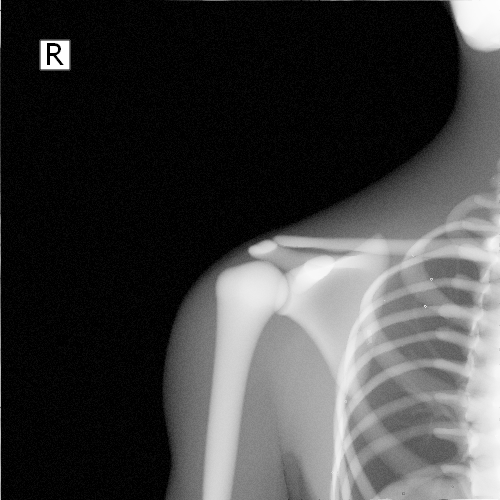
\includegraphics[width=\linewidth]{IMG/xraynointernal.png}}
        \caption{Tejido óseo original del \emph{ZygoteBody}$^{TM}$ Masculino\label{subfig:nointernal}.}
    \end{subfigure}
    \null\hfill
     \begin{subfigure}[b]{0.45\linewidth}
        \centering
        {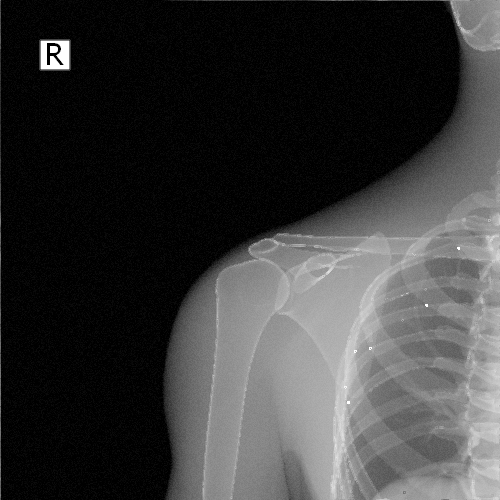
\includegraphics[width=\linewidth]{IMG/xrayinternal.png}}
        \caption{Resultado de la inclusión del tejido interior de los huesos.}
    \end{subfigure}
    \caption{\label{fig:bonecompare} Comparativa entre una el mallado original de \emph{ZygoteBody}$^{TM}$ Masculino y la introducción del tejido trabecular en los huesos.}
   \end{figure}


Frente a un libro tradicional de proyecciones radiológicas donde se muestran unas imágenes estáticas, 
el simulador desarrollado permite al estudiante interaccionar con un modelo anatómico.
Como se puede observar en la figura \ref{fig:xraycomp}, se ha seleccionado una proyección radiológica procedente de \cite{carver2012medical} y se ha procedido a replicar la misma posición en la herramienta. El simulador ofrece la ventaja de poder obtener más imágenes y/o proyecciones adicionales del mismo paciente virtual, que resultaría imposible si quisiese obtenerse de un paciente real debido a su peligrosidad. Por tanto, se  permite a profesores y estudiantes practicar de manera más extensa con un mismo modelo anatómico en un entorno completamente seguro.


% \begin{figure}[tb]
% \centering
% 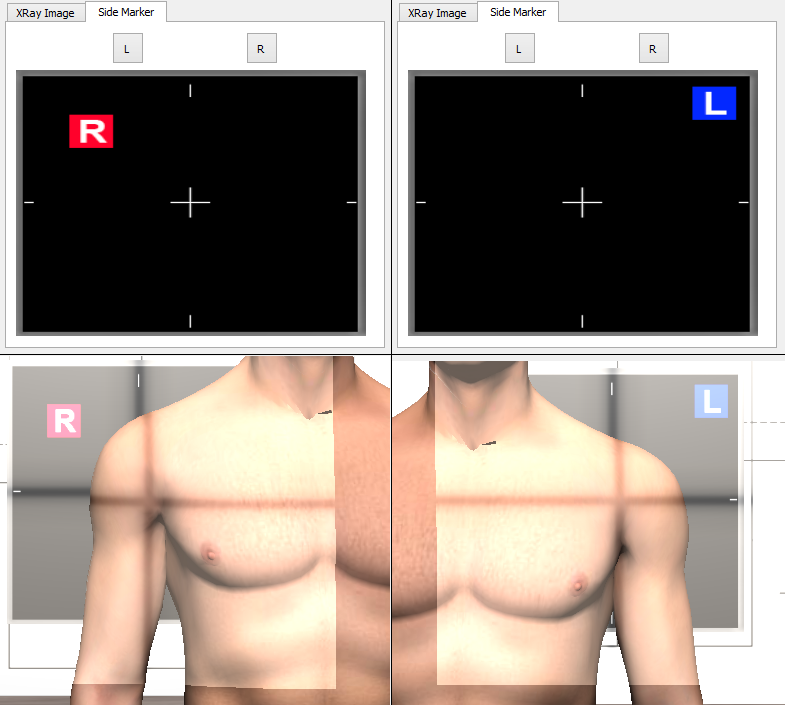
\includegraphics[width=0.5\linewidth]{IMG/side.png}
% \caption{\label{fig:xraycomp} Comparativa entre una imagen del libro\cite{carver2012medical} y la imagen resultante de la herramienta. }
% \end{figure}

\begin{figure}[ht]
    \begin{subfigure}[b]{0.45\linewidth}
        \centering
        {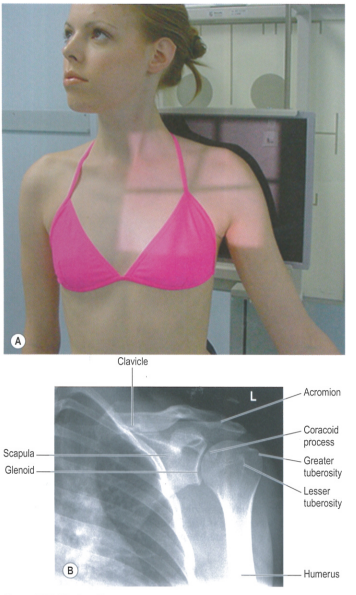
\includegraphics[width=\linewidth]{IMG/carvershoulder.PNG}}
        \caption{Imagen cortesía de E. Carver, B. Carver y Elsevier Health Sciences~\cite{carver2012medical}.}
    \end{subfigure}
    \null\hfill
     \begin{subfigure}[b]{0.45\linewidth}
        \centering
        {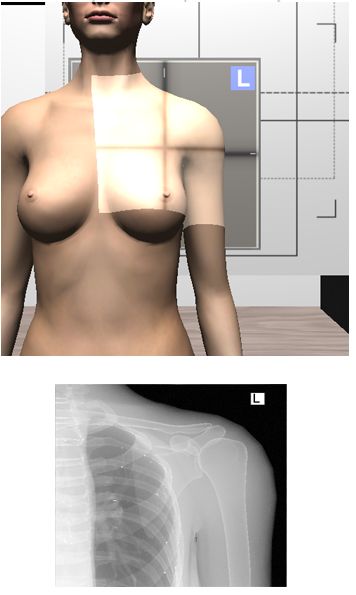
\includegraphics[width=\linewidth]{IMG/XRayshoulder3.png}}
        \caption{Proyección anteroposterior del hombro replicada en el simulador.}
    \end{subfigure}
    \caption{\label{fig:xraycomp} Comparativa entre una imagen del libro \cite{carver2012medical} y la imagen resultante del simulador.}
   \end{figure}

Otra muestra de las ventajas del simulador frente a los materiales educativos tradicionales se puede observar en la figura \ref{fig:diseaseresult}. En esta ocasión, el simulador permite generar variaciones del mismo modelo anatómico. Con ello, se pueden enseñar como se manifestaría una enfermedad y, por tanto, ayudar a la interpretación de una imagen radiológica en el futuro. Cambiando unos pocos parámetros, el simulador permite cambiar entre un tejido sano o enfermo. Incluso puede ser interesante que los estudiantes puedan observar como se distinguen objetos extraños cuando se encuentran dentro de la anatomía del paciente. A través de la \ac{IU}, se podrá rotar el paciente virtual para conseguir una radiografía desde distintos ángulos de vista frente a la imagen estática mostrada en los archivos educativos y repositorios.

\begin{figure}[ht]
\begin{subfigure}[b]{0.3\linewidth}
        \centering
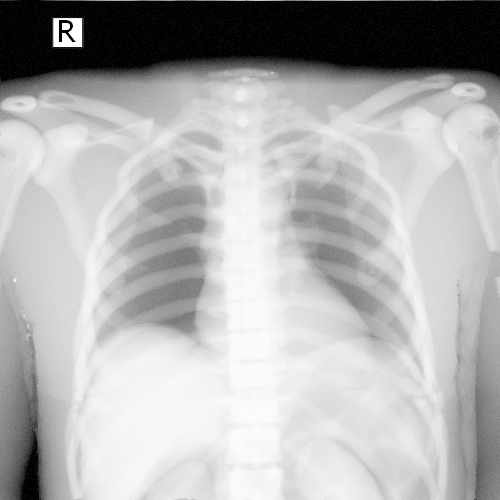
\includegraphics[width=\linewidth]{IMG/HVPForeign.png}
        \caption{Imagen  de \emph{Segmented Inner Organs} \cite{VoxelMan}.}
    \end{subfigure}
    \null\hfill
    \begin{subfigure}[b]{0.3\linewidth}
        \centering
        {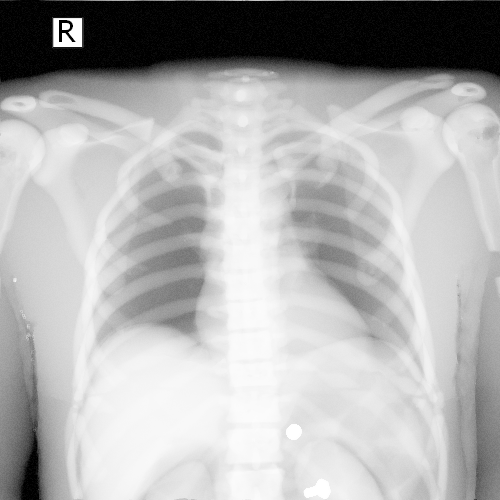
\includegraphics[width=\linewidth]{IMG/HVPNormal.png}}
        \caption{Objetos extraños en el estómago.}
    \end{subfigure}
    \null\hfill
     \begin{subfigure}[b]{0.3\linewidth}
        \centering
        {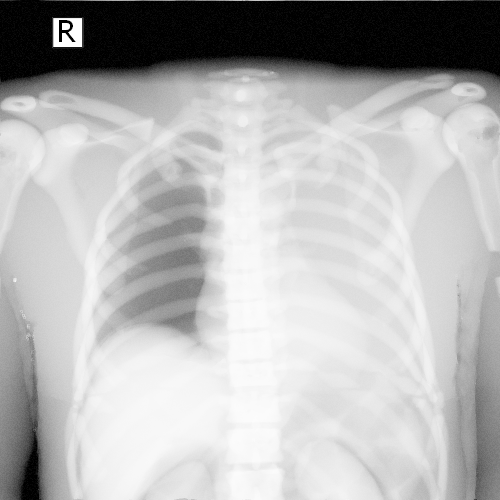
\includegraphics[width=\linewidth]{IMG/HVPLung.png}}
        \caption{Simulación de pulmón izquierdo colapsado.}
    \end{subfigure}
    \caption{\label{fig:diseaseresult} Un usuario puede ilustrar diferentes ejemplos con el mismo paciente virtual.}
   \end{figure}

% \begin{figure}[tb]
% \centering
% 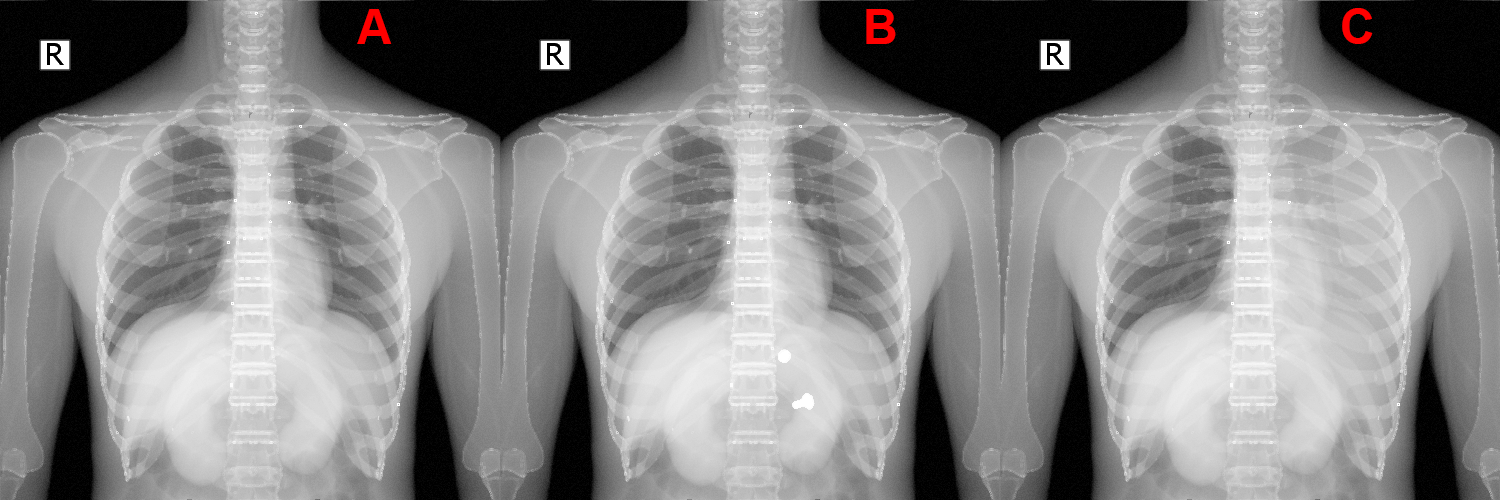
\includegraphics[width=0.5\linewidth]{IMG/disease.png}
% \caption{\label{fig:resultdisease}Usuarios pueden probar diferentes casos. A: Anatomía normal. B: Objetos extraños en el estómago. C: Pulmón izquierdo colapsado. }
% \end{figure}

\clearpage
\subsection{Rendimiento}

Al igual que en la sección \ref{posing:result}, el cauce de animación propuesto se han delegado las etapas más costosas computacionalmente a un preproceso. Esto permite que, junto con los datos auxiliares generados, la selección de poses y por tanto el simulador pueda ser interactivo. A su vez, ambos algoritmos (posicionador de pacientes virtuales y la librería de simulación de rayos X) comparten memoria en \acs{GPU} para mejorar la eficiencia y poder ejecutarse interactivamente. En el peor de los casos, el modelo de \emph{ZygoteBody}$^{TM}$ y su malla de tetraedros se componen de $1.5$ millones de vértices y $2.5$ millones de tetraedros. En la tabla \ref{tab:xraytime}, se pueden consultar el tiempo empleado en milisegundos por cada etapa utilizando los modelos \emph{ZygoteBody}$^{TM}$ Masculino y Femenino, Anatomium y la representación superficial del Segmented Inner Organs. La tabla muestra los valores máximos y mínimos de tiempo que tarda en ejecutar cada módulo, siendo capaz de mantenerse por encima de las $25$ imágenes por segundo.





\begin{table}[ht]
\centering
\caption{Valores máximos y mínimos del tiempo de \emph{renderizado} y generación de las imágenes de rayos X. Medido en milisegundos. }
\begin{tabular}{|c|x{5cm}|c|}
%\multirow{2}{*}{\textbf{Model}} & \multicolumn{2}{c}{\textbf{Interactive stage}} & \multirow{2}{*}{\textbf{Optimization}} \\
\hline
\textbf{Modelo}&\textbf{Algoritmo de posicionamiento} &\textbf{gVirtualXRay}  \\ 
\hline
\emph{ZygoteBody}$^{TM}$ Masculino  & 25-16 & 22-18 \\ 
\hline
\emph{ZygoteBody}$^{TM}$ Femenino  & 29-21  & 23-17    \\ 
\hline
Anatomium   & 20-13 & 21-18 \\ 
\hline
Segmented Inner Organs   & 17-08 & 15-12 \\ 
\hline
\end{tabular}
\label{tab:xraytime}
\end{table}

%Para alcanzar estas tasas de refresco, el algoritmo propuesto delega las operaciones más complejas a un proceso previo descrito en la sección \ref{posing:result}.
%El mayor consumo de tiempo viene dado por el proceso previo del algoritmo propuesto (ver sección \ref{posing:result}) y la complejidad del modelo virtual, que en el caso de \emph{ZygoteBody}$^{TM}$ toma menos de 7 minutos.

\subsection{Validación}
\label{xray:validacion}
Para comprobar la validez aparente y de contenido del simulador se ha diseñado un estudio, donde se ha pedido a los participantes observar una serie de vídeos que describían las funcionalidades del simulador. A continuación, se les hacía unas preguntas referentes al vídeo y al simulador. Se ha seleccionado como población objetivo el conjunto de especialistas relacionados con la técnica de radiología. En los cuales, se buscaba contar con la opinión de estudiantes y profesionales, incluyendo varios países. La encuesta se puede consultar en el anexo \ref{anexo:cuestionarioxray}.
%
Al finalizar la encuesta, se han registrado 18 participaciones (con un $50\%$ de mujeres y hombres): donde 16 de ellos han seleccionado la categoría profesional \emph{técnico en radiología} mientras que el resto son otro tipo de profesional médico que trabajan con imágenes radiológicas; de 4 países diferentes (15 de Reino Unido, 1 de Francia, 1 de Canadá y 1 de España); con años de práctica de radiología entre 1 y 40 años (ver figura \ref{fig:year}).
%
En el formulario, se incluía una pregunta sobre la confianza del participante a la hora de tomar una imagen de rayos X. Tal y como se ve en la figura \ref{fig:confident}, muestra un amplio número de participantes que reflejan una alta confianza en sus habilidades.
%
Por otra parte, también se incluía la pregunta sobre la confianza del participante en sus habilidades para interpretar la radiografía con fines de diagnóstico médico. En la figura \ref{fig:interpreting} se muestra el histograma con los resultados. En este caso, hay más variabilidad en las respuestas.


\begin{figure}[ht]
        \centering
        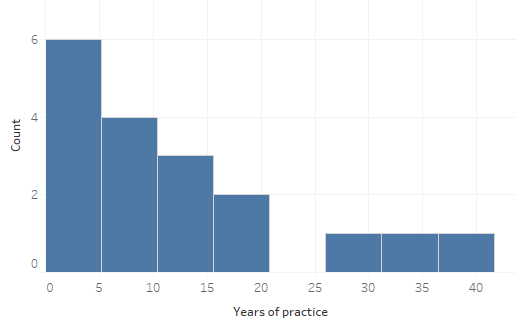
\includegraphics[width=0.75\linewidth]{IMG/years.png}
        {
         \caption{\label{fig:year}Histograma de los años de experiencia de los participantes.}
        }
       
    \end{figure}
     \begin{figure}[ht]
        \centering
        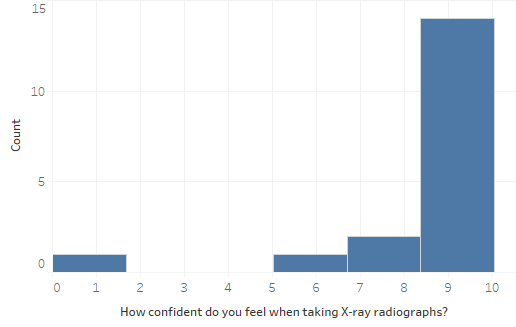
\includegraphics[width=0.75\linewidth]{IMG/confident.png}{
        
        \caption{\label{fig:confident}Histograma de las respuestas a la pregunta sobre como de confiados se sienten al tomar una radiografía.}
        }
    \end{figure}
   
     \begin{figure}[ht]
        \centering
        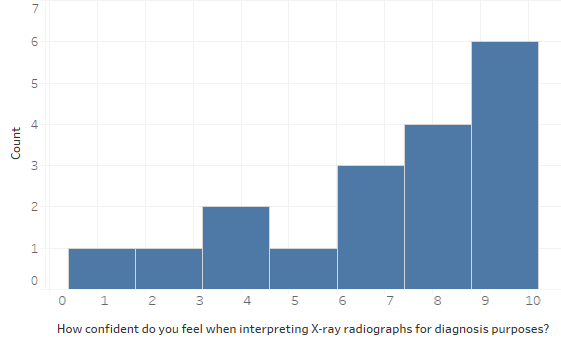
\includegraphics[width=0.75\linewidth]{IMG/interpreting.png}{
        \caption{\label{fig:interpreting}Histograma de las respuestas a la pregunta sobre como de confiados se sienten al interpretar una radiografía con fines diagnósticos.}
        }
    \end{figure}


\subsubsection{Validez aparente}

En cuanto a la validez aparente, se han incluido en la encuesta las preguntas de la tabla \ref{tab:facevalidity}. Estas preguntas eran de tipo \emph{Likert}, donde se podía responder con valores comprendidos desde 1 (Nada de acuerdo) hasta 5 (Muy de acuerdo). 

En la figura \ref{fig:facevalidity}, se pueden observar los resultados por cada pregunta mostrados en porcentaje de respuestas. Es destacable que en general, hay al menos un 60\% de respuestas positivas en todas las preguntas y ninguna respuesta completamente negativa, excepto la pregunta F3. Esta pregunta trata sobre la descripción de los pasos que debe realizar un médico cuando está realizando el procedimiento. Cuando en la sección \ref{art:xraysim} se describió los pasos del procedimiento de proyecciones radiológicas, en el propio libro \cite{manualpractico} se advertía sobre las posibles variaciones dependiendo del lugar de trabajo.  

\begin{figure}[hb]
    \centering
    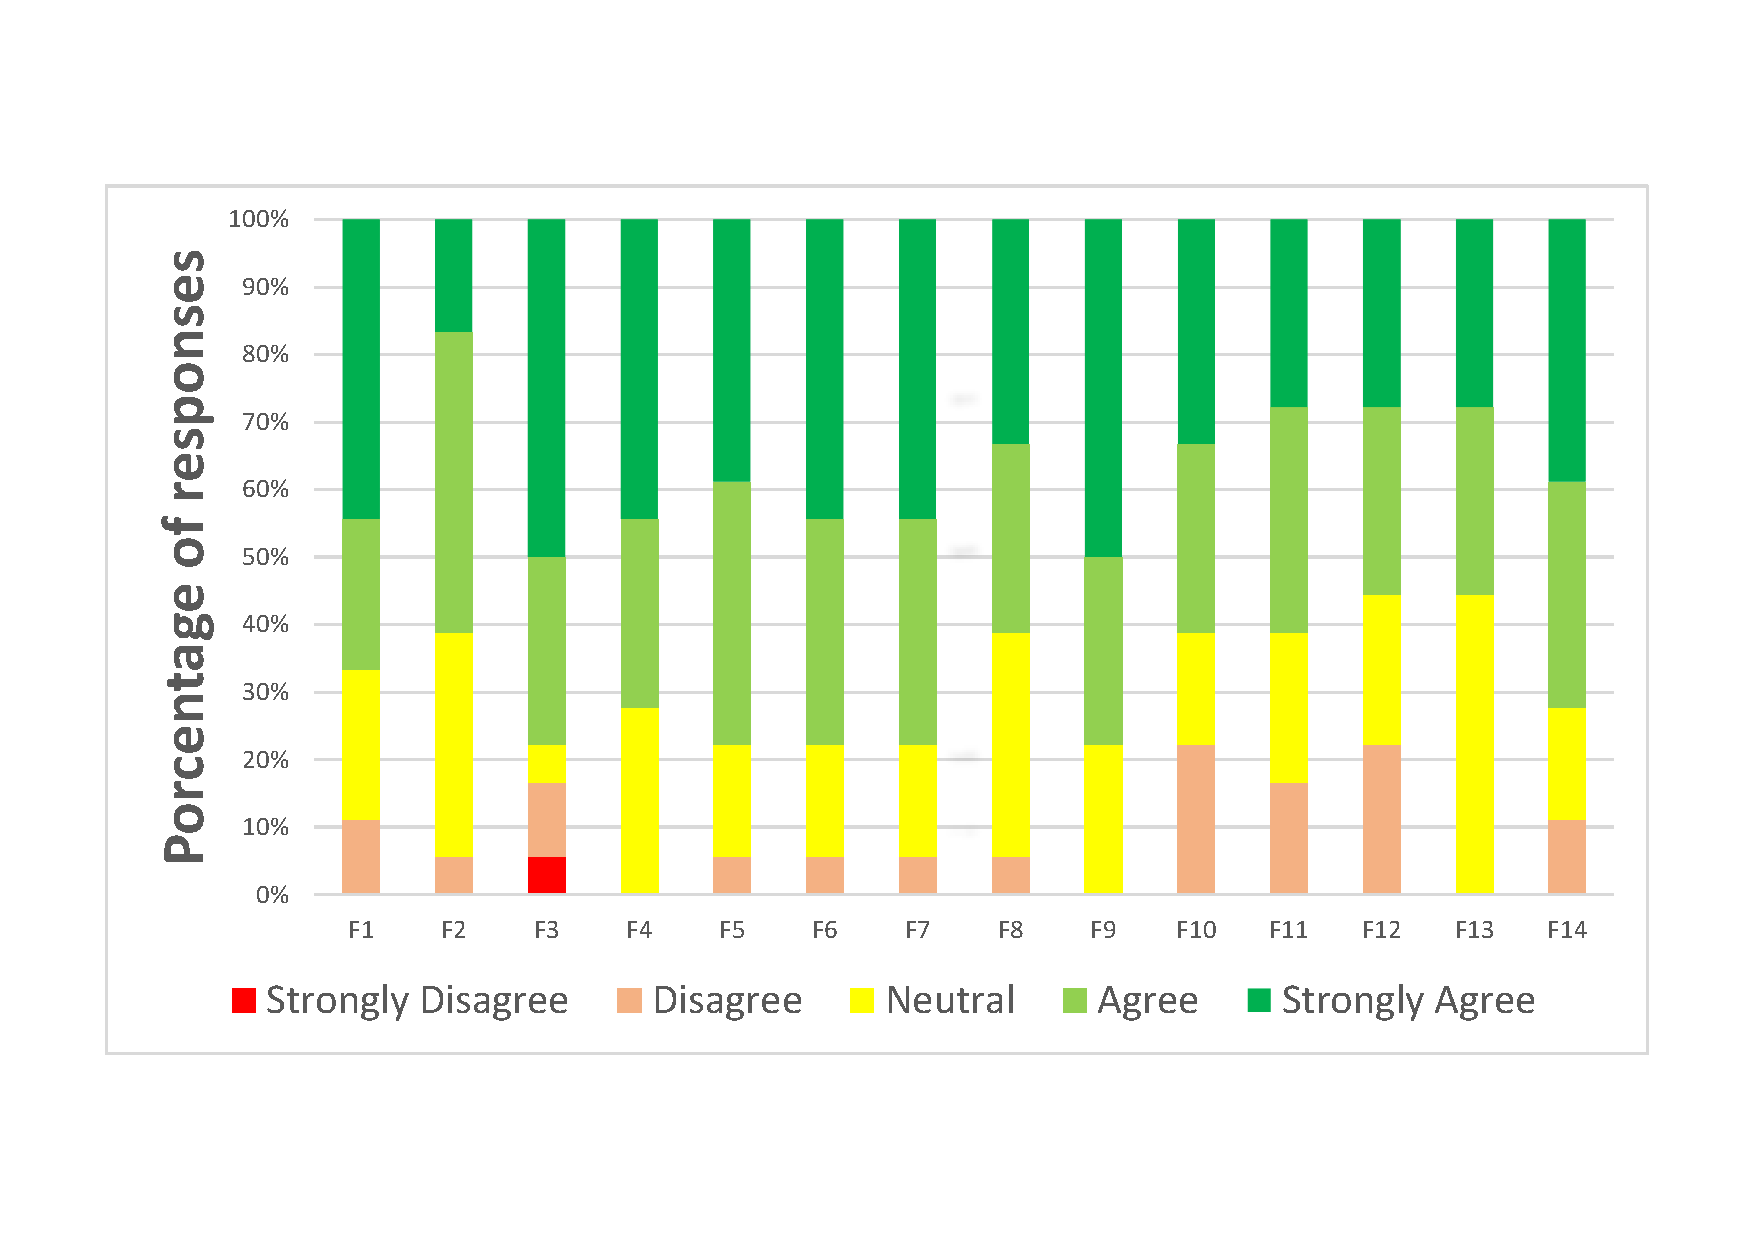
\includegraphics[trim={15mm 25mm 15mm 25mm},clip,width=\linewidth]{IMG/facevalidty.pdf}
    \caption{Gráfica que muestra los porcentajes de respuestas tipo \emph{Likert} en las preguntas de validez aparente.}
    \label{fig:facevalidity}
\end{figure}


\begin{table}[hb]
    \centering
    \begin{tabular}{lp{14cm}}
    \hline
    \multicolumn{2}{c}{Face validity }
    \\
    \hline
    F1:     &  The patient model before selecting the posing is visually realistic.  \\
    F2:     & The deformation of the patient’s internal anatomy is visually realistic.  \\
    F3:     & The previously described steps characterize the procedure in a realistic way.  \\
    F4:     & The placement of the side markers on the x-ray image is visually realistic.   \\
    F5:     & The changes in the final x-ray image due to the adjustment of the beam direction and FRD are visually realistic.  \\
    F6:     & The adjustment of the centre is visually realistic. \\
    F7:     & The changes in the final x-ray image due to the collimation adjustment are visually realistic.  \\
    F8:     & The changes in the final x-ray image due to beam energy configuration are visually realistic.  \\
    F9:     & In general, the changes in the final x-ray image due to modification of the different parameters are visually realistic. \\
    F10:     & The adjustment of the brightness and contrast settings is visually realistic.  \\
    F11:     & The use of image filters is visually realistic.  \\
    F12:     & The simulation of diseases is visually realistic.  \\
    F13:     & The inclusion of foreign objects in the virtual patient is visually realistic.  \\
    F14:     & Generally speaking, the simulator is visually realistic.  \\
    
    \hline
    \end{tabular}
    \caption{Preguntas realizadas para la validez aparente.}
    \label{tab:facevalidity}
\end{table}
\clearpage
\subsubsection{Validez de contenido}

Las preguntas relativas a la validez de contenido se pueden leer en la tabla \ref{tab:contentvalidity}. Al igual que el caso anterior, estas preguntas eran de tipo \emph{Likert}, donde se podía responder con valores comprendidos desde 1 (Nada de acuerdo) hasta 5 (Muy de acuerdo).

En la figura \ref{fig:contentvalidity}, se pueden observar los resultados por cada pregunta mostrados en porcentaje de respuestas. Los resultados son parecidos a la validez de apariencia, donde se han registrado al menos un 60\% de respuestas positivas en todas las preguntas. 

\begin{figure}[hb]
    \centering
    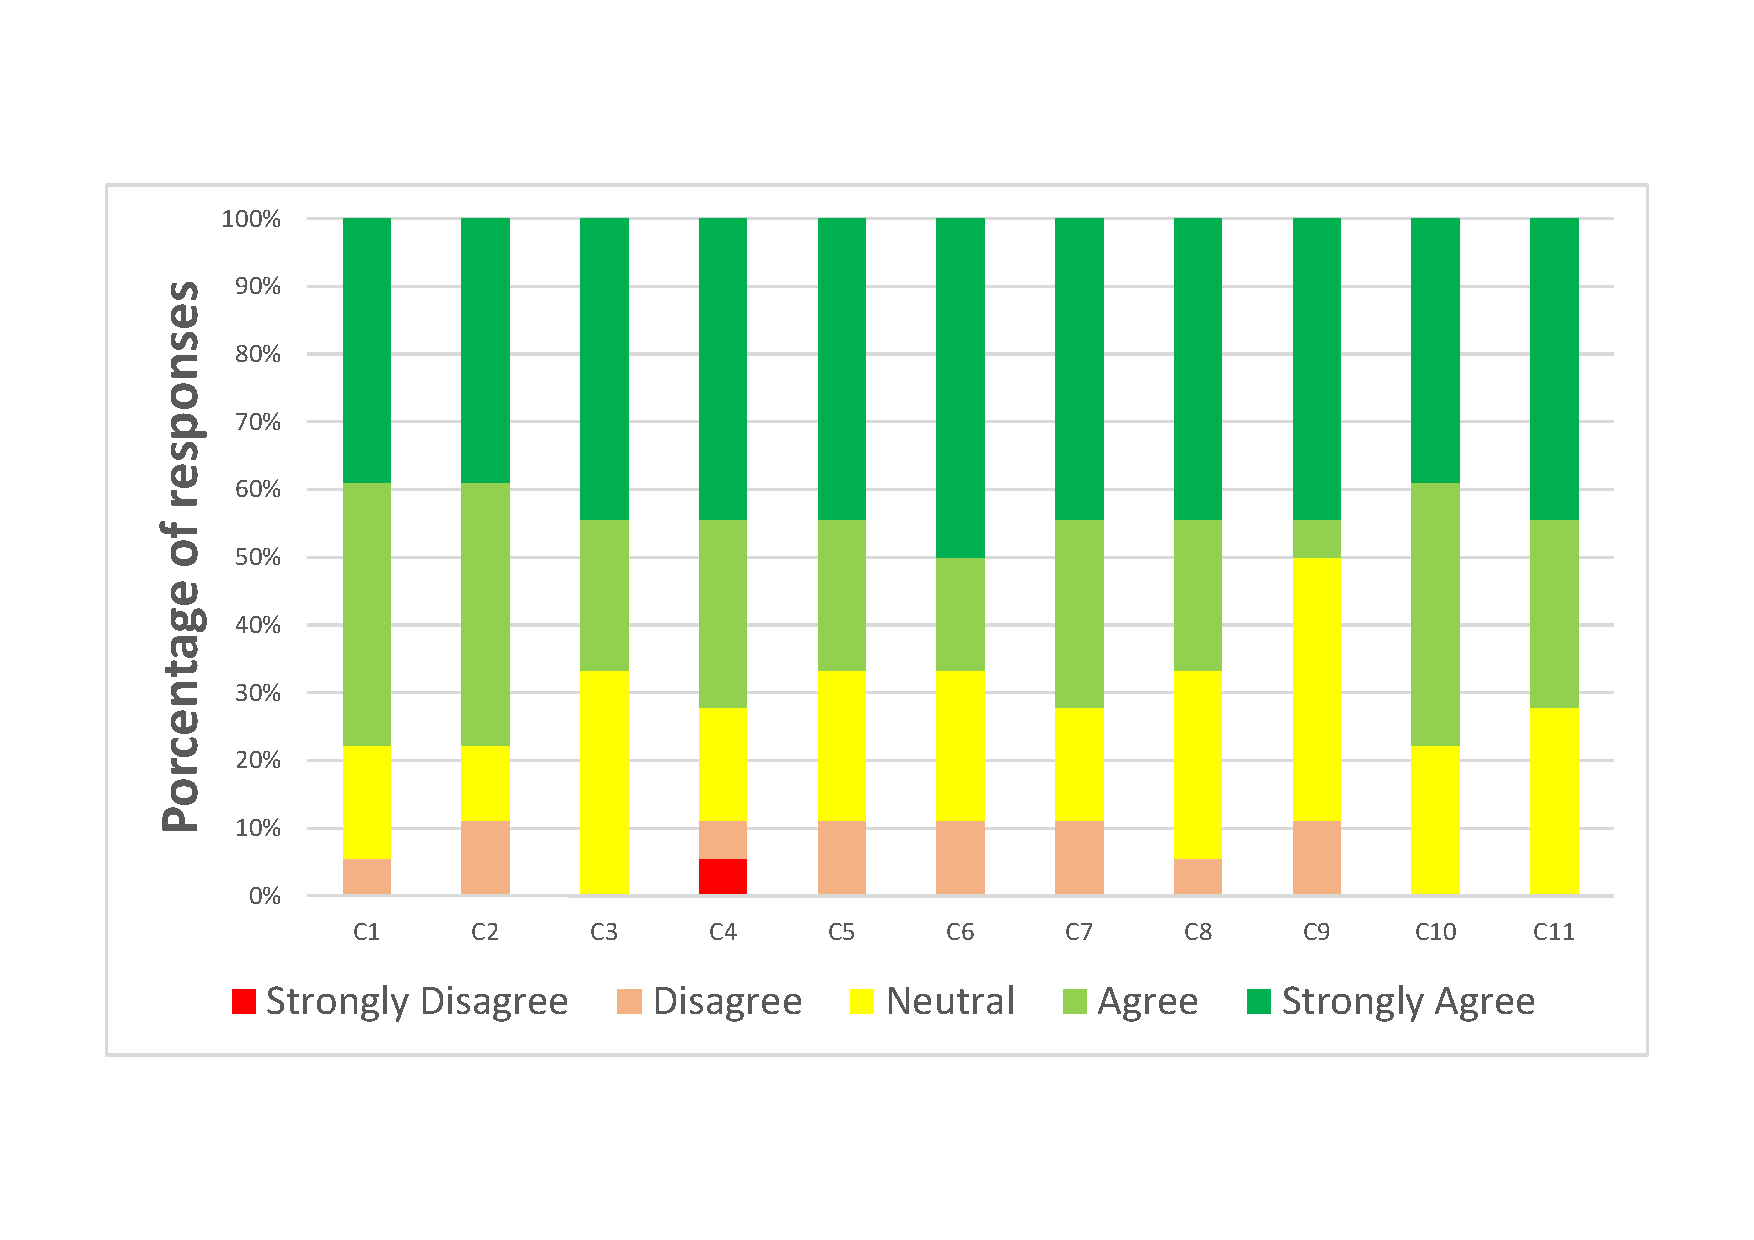
\includegraphics[trim={15mm 25mm 15mm 25mm},clip,width=\linewidth]{IMG/contentvalidty.pdf}
    \caption{Gráfica que muestra los porcentajes de respuestas tipo \emph{Likert} en las preguntas de validez de contenido.}
    \label{fig:contentvalidity}
\end{figure}




\begin{table}[ht]
    \centering
    \begin{tabular}{lp{14cm}}
    \hline
    \multicolumn{2}{c}{Content validity }
    \\
    \hline
    C1:     &  Selecting the patient pose from a set of predefined ones is useful for self-guided training.  \\
    C2:     & Selecting the patient manually is useful for self-guided training.   \\
    C3:     & Selecting the patient pose from a set of predefined ones is useful to teach the procedure.   \\
    C4:     & Selecting the patient manually is useful for teaching purposes (e.g. for live demonstration in the lecture theatre).    \\
    C5:     &  Regarding the previously described steps, the simulator is useful to teach the procedure.  \\
    C6:     & Regarding the previously described steps, the simulator is useful for self-guided training.  \\
    C7:     & In general, digital image manipulation of the X-ray image is useful for self-guided training and teaching.  \\
    C8:     & Regarding the functionality described, this is useful to teach the procedure.   \\
    C9:     & Regarding the functionality described, the simulator is useful  for self-guided training.  \\
    C10:     & Generally speaking, the simulator is suitable is useful as a teaching tool.   \\
    C11:     & Generally speaking, the simulator is suitable for self-guided training.   \\
    \hline
    \end{tabular}
    \caption{Preguntas realizadas para la validez de contenido.}
    \label{tab:contentvalidity}
\end{table}

Los resultados obtenidos sugieren que el simulador de radiología diagnóstica es visualmente realista. En general, todas las funcionalidades han obtenido una valoración positiva. Además, aunque se registraron pocos comentarios libres, estos comentarios eran positivos. Esto sugiere que, aunque los modelos anatómicos presenten problemas de calidad, el algoritmo de posicionamiento de pacientes virtuales genera posturas útiles para el entrenamiento. A la vista de la mayoría de participantes, el simulador proporciona las funcionalidades y el realismo necesarios para entrenar el procedimiento. En cuanto a la validez de contenido, las respuestas han sido mayormente positivas, indicando que el simulador es útil para la enseñanza y entrenamiento del procedimiento. 

% \subsection{Discusión}
% \label{xray:discusion}
% Los resultados del simulador muestran una herramienta educativa muy completa que puede ser usada como material complementario para los estudiantes de radiología. La aplicación proporciona un entorno seguro e interactivo para comprobar todo tipo de situaciones. El posicionador de pacientes virtuales permite una interacción en tiempo real con la posibilidad de generar una cantidad de variaciones anatómicas superior a los métodos clásicos como pueden ser los libros o archivos de casos y a los simuladores introducidos en la sección \ref{art:entrenamiento}.

% Esta herramienta también demuestra la versatilidad del algoritmo presentado en esta tesis, ya que puede ser incorporado en cualquier simulador que necesite deformaciones plausibles en tiempos interactivos, permitiendo que sea el usuario quien decida la posición final.

% Aunque la aplicación se ha diseñado para satisfacer las necesidades de los radiólogos, presenta ciertas limitaciones respecto al procedimiento de diagnóstico por imagen. Existen cuestiones relacionadas con la preparación del paciente para el procedimiento que no pueden ser cubiertas por el simulador, entre ellas las siguientes:

% \begin{itemize}
%     \item Se recomienda utilizar un lenguaje apropiado y efectivo en la comunicación con los pacientes que no es posible recoger por el simulador.
%     \item No se representa la necesidad de indicar al paciente acerca de quitarse prendas u objetos que afecten al área de examen.
%     \item No se practican las recomendaciones en cuanto al uso de protectores de plomo para pacientes y profesionales.
%     \item Otras comprobaciones que implican condiciones médicas o protocolarias como embarazo, identificación del paciente, etc...
% \end{itemize}

En resumen, a la vista de los resultados de las validaciones realizadas, los profesionales han valorado positivamente el simulador. Esto confirma que el simulador puede ser utilizado como herramienta de clase por parte de los profesores, como por el alumnado para practicar el procedimiento. 
